\documentclass{ximera}
\input{../preamble.tex}

\title{Essential Vocabulary} \license{CC BY-NC-SA 4.0}



\begin{document}
\begin{abstract}
\end{abstract}
\maketitle


\begin{onlineOnly}
\section*{Essential Vocabulary}
Here is a  \href{https://quizlet.com/880918143/chapter-2-vocabulary-flash-cards/?i=y06sd&x=1jqt}{link to a list of these terms on Quizlet}
\end{onlineOnly}

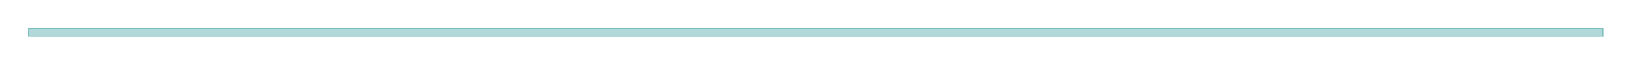
\begin{tikzpicture}[scale=1]
   \filldraw[teal, opacity=0.3](0,0)--(20,0)--(20,0.1)--(0,0.1)--cycle;
 \end{tikzpicture}


Augmented matrix
\begin{expandable}
    Every linear system 
$$\begin{array}{ccccccccc}
      a_{11}x_1 &+ &a_{12}x_2&+&\ldots&+&a_{1n}x_n&= &b_1 \\
	 a_{21}x_1 &+ &a_{22}x_2&+&\ldots&+&a_{2n}x_n&= &b_2 \\
     &&&&\vdots&&&& \\
     a_{m1}x_1 &+ &a_{m2}x_2&+&\ldots&+&a_{mn}x_n&= &b_m
    \end{array}$$
    can be written in the \dfn{augmented matrix form} as follows:
    $$\left[\begin{array}{cccc|c}  
 a_{11}&a_{12}&\ldots&a_{1n}&b_1\\a_{21}&a_{22}&\ldots&a_{2n}&b_2\\\vdots&\vdots&\ddots&\vdots&\vdots\\a_{m1}&a_{m2}&\ldots&a_{mn}&b_m
 \end{array}\right]$$
 The array to the left of the vertical bar is called the \dfn{coefficient matrix} of the linear system and is often given a capital letter name, like $A$.  The vertical array to the right of the bar is called a \dfn{constant vector}.
 $$A=\begin{bmatrix}a_{11}&a_{12}&\ldots&a_{1n}\\a_{21}&a_{22}&\ldots&a_{2n}\\\vdots&\vdots&\ddots&\vdots\\a_{m1}&a_{m2}&\ldots&a_{mn}\end{bmatrix}\quad\text{and}\quad\vec{b}=\begin{bmatrix}b_1\\b_2\\\vdots\\b_m\end{bmatrix}$$
We will sometimes use the following notation to represent an augmented matrix.

$$\left[\begin{array}{c|c}  
 A & \vec{b}\\
 \end{array}\right]$$
\end{expandable}

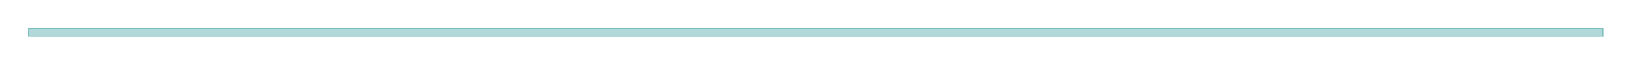
\begin{tikzpicture}[scale=1]
   \filldraw[teal, opacity=0.3](0,0)--(20,0)--(20,0.1)--(0,0.1)--cycle;
 \end{tikzpicture}


Back substitution
\begin{expandable}
When a matrix is in row-echelon form, we can compute the solution to the system by starting from the last equation and working backwards.  This process is known as \dfn{back substitution}.
\end{expandable}


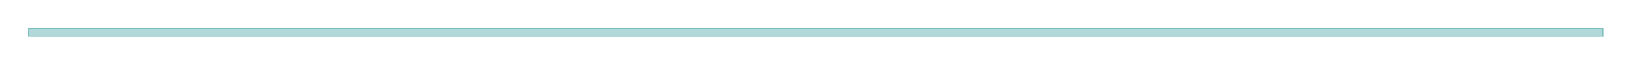
\begin{tikzpicture}[scale=1]
   \filldraw[teal, opacity=0.3](0,0)--(20,0)--(20,0.1)--(0,0.1)--cycle;
 \end{tikzpicture}

Coefficient matrix
\begin{expandable}
    A \dfn{coefficient matrix} is a matrix whose entries are the coefficients of a system of linear equations.  For the system $$\begin{array}{ccccccccc}
      a_{11}x_1 &+ &a_{12}x_2&+&\ldots&+&a_{1n}x_n&= &b_1 \\
	 a_{21}x_1 &+ &a_{22}x_2&+&\ldots&+&a_{2n}x_n&= &b_2 \\
     &&&&\vdots&&&& \\
     a_{m1}x_1 &+ &a_{m2}x_2&+&\ldots&+&a_{mn}x_n&= &b_m
    \end{array},$$ 
    the \dfn{coefficient matrix} is $A=\begin{bmatrix}a_{11}&a_{12}&\ldots&a_{1n}\\a_{21}&a_{22}&\ldots&a_{2n}\\\vdots&\vdots&\ddots&\vdots\\a_{m1}&a_{m2}&\ldots&a_{mn}\end{bmatrix}$.
\end{expandable}

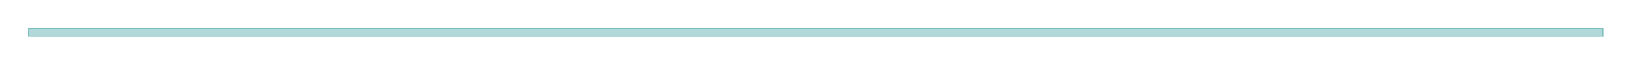
\begin{tikzpicture}[scale=1]
   \filldraw[teal, opacity=0.3](0,0)--(20,0)--(20,0.1)--(0,0.1)--cycle;
 \end{tikzpicture}

Consistent system
\begin{expandable}
    A system of equations that has at least one solution.
\end{expandable}

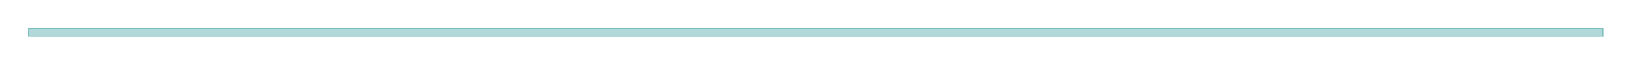
\begin{tikzpicture}[scale=1]
   \filldraw[teal, opacity=0.3](0,0)--(20,0)--(20,0.1)--(0,0.1)--cycle;
 \end{tikzpicture}

Convergence
\begin{expandable}
    when the iterates of an iterative method approach a solution
\end{expandable}

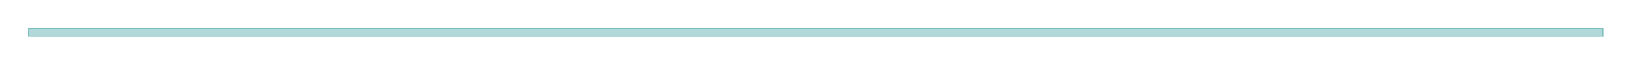
\begin{tikzpicture}[scale=1]
   \filldraw[teal, opacity=0.3](0,0)--(20,0)--(20,0.1)--(0,0.1)--cycle;
 \end{tikzpicture}

Divergence
\begin{expandable}
    when the iterates of an iterative method fail to approach a solution
\end{expandable}

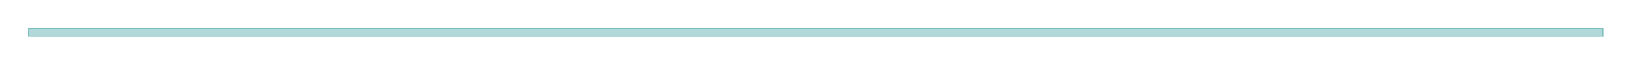
\begin{tikzpicture}[scale=1]
   \filldraw[teal, opacity=0.3](0,0)--(20,0)--(20,0.1)--(0,0.1)--cycle;
 \end{tikzpicture}


Elementary row operations
\begin{expandable}
    The following three operations performed on a linear system are called \dfn{elementary row operations}.
\begin{enumerate}
\item Switching the order of equations (rows) $i$ and $j$:
$$R_i\leftrightarrow R_j$$
\item Multiplying both sides of equation (row) $i$ by the same non-zero constant, $k$, and replacing equation $i$ with the result:
$$kR_i\rightarrow R_i$$
\item Adding $k$ times equation (row) $i$ to equation (row) $j$, and replacing equation $j$ with the result:
$$R_j+kR_i\rightarrow R_j$$
\end{enumerate}
\end{expandable}

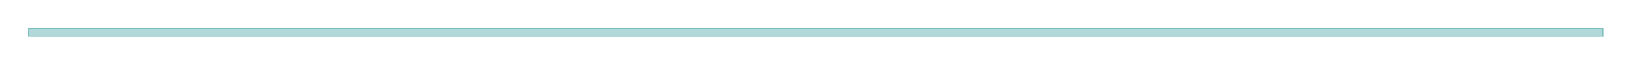
\begin{tikzpicture}[scale=1]
   \filldraw[teal, opacity=0.3](0,0)--(20,0)--(20,0.1)--(0,0.1)--cycle;
 \end{tikzpicture}

Equivalent systems
\begin{expandable}
    Linear systems are called \dfn{equivalent} if they have the same solution set.
\end{expandable}

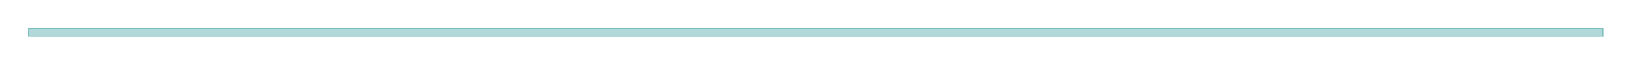
\begin{tikzpicture}[scale=1]
   \filldraw[teal, opacity=0.3](0,0)--(20,0)--(20,0.1)--(0,0.1)--cycle;
 \end{tikzpicture}

Free variable
\begin{expandable}
    When a linear system is in row-echelon form, the variables corresponding to columns that do not have any leading coefficients (if there are any) are known as \dfn{free variables}.
\end{expandable}

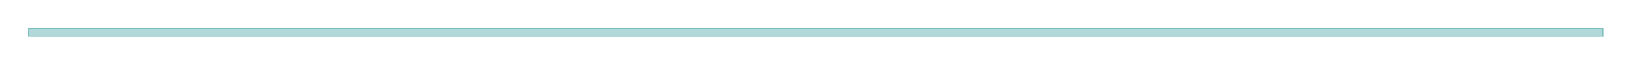
\begin{tikzpicture}[scale=1]
   \filldraw[teal, opacity=0.3](0,0)--(20,0)--(20,0.1)--(0,0.1)--cycle;
 \end{tikzpicture}

 Gauss-Jordan elimination 
\begin{expandable}
    The process of using the elementary row operations on a matrix to transform it into reduced row-echelon form is called \dfn{Gauss-Jordan elimination}.
\end{expandable}


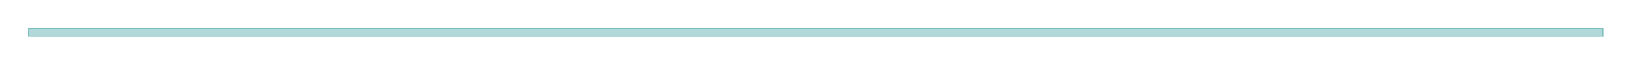
\begin{tikzpicture}[scale=1]
   \filldraw[teal, opacity=0.3](0,0)--(20,0)--(20,0.1)--(0,0.1)--cycle;
 \end{tikzpicture}


Gauss-Seidel Method
\begin{expandable}
    An iterative method for solving linear systems that is a refinement of the Jacobi method, where we use computed values of variables alternately for quicker convergence.
\end{expandable}


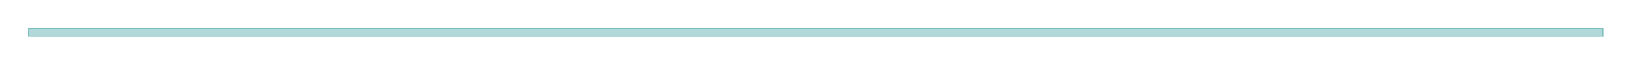
\begin{tikzpicture}[scale=1]
   \filldraw[teal, opacity=0.3](0,0)--(20,0)--(20,0.1)--(0,0.1)--cycle;
 \end{tikzpicture}

 Gaussian elimination
\begin{expandable}
    The process of using the elementary row operations on a matrix to transform it into row-echelon form is called \dfn{Gaussian Elimination}.
\end{expandable}


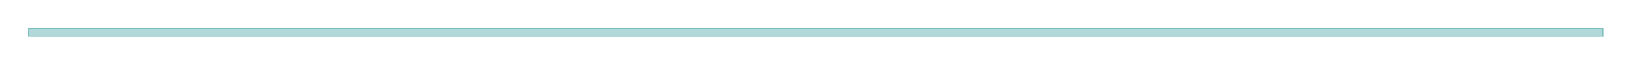
\begin{tikzpicture}[scale=1]
   \filldraw[teal, opacity=0.3](0,0)--(20,0)--(20,0.1)--(0,0.1)--cycle;
 \end{tikzpicture}

Inconsistent system
\begin{expandable}
    A system of equations that has no solution.
\end{expandable}


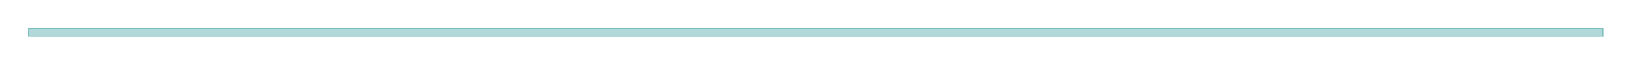
\begin{tikzpicture}[scale=1]
   \filldraw[teal, opacity=0.3](0,0)--(20,0)--(20,0.1)--(0,0.1)--cycle;
 \end{tikzpicture}

Jacobi's method
\begin{expandable}
    An iterative method for solving a system of equations where one variable is isolated in each equation in order to compute the coordinate of the next iterate.
\end{expandable}

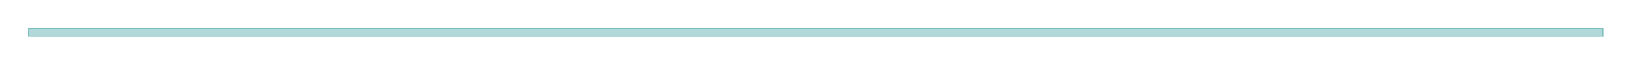
\begin{tikzpicture}[scale=1]
   \filldraw[teal, opacity=0.3](0,0)--(20,0)--(20,0.1)--(0,0.1)--cycle;
 \end{tikzpicture}

Leading entry (leading 1)
\begin{expandable}
    The first non-zero entry in a row of a matrix (when read from left to right) is called the \dfn{leading entry}.  When the leading entry is 1, we refer to it as a \dfn{leading 1}.
\end{expandable}

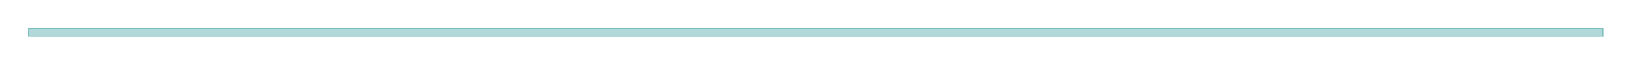
\begin{tikzpicture}[scale=1]
   \filldraw[teal, opacity=0.3](0,0)--(20,0)--(20,0.1)--(0,0.1)--cycle;
 \end{tikzpicture}

Linear equation
\begin{expandable}
    A \dfn{linear equation} in variables $x_1, \ldots, x_n$ is an equation that can be written in the form
$$a_1x_1+a_2x_2+\ldots +a_nx_n=b$$
where $a_1,\ldots ,a_n$ and $b$ are constants.
\end{expandable}


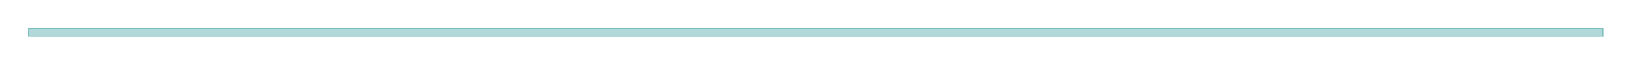
\begin{tikzpicture}[scale=1]
   \filldraw[teal, opacity=0.3](0,0)--(20,0)--(20,0.1)--(0,0.1)--cycle;
 \end{tikzpicture}

Pivot
\begin{expandable}
    In Gaussian elimination, an entry chosen to become a leading coefficient used to get zeros in the remaining rows.
\end{expandable}

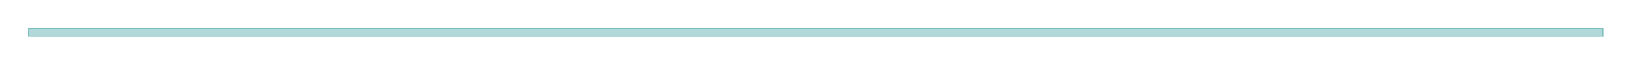
\begin{tikzpicture}[scale=1]
   \filldraw[teal, opacity=0.3](0,0)--(20,0)--(20,0.1)--(0,0.1)--cycle;
 \end{tikzpicture}


Rank of a matrix
\begin{expandable}
    The \dfn{rank} of matrix $A$, denoted by $\mbox{rank}(A)$, is the number of nonzero rows that remain after we reduce $A$ to row-echelon form by elementary row operations.
\end{expandable}

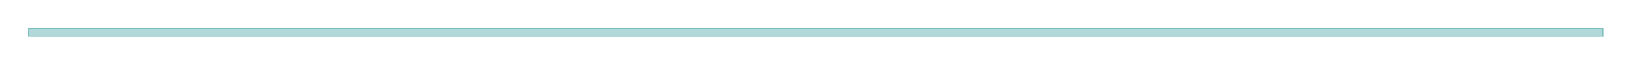
\begin{tikzpicture}[scale=1]
   \filldraw[teal, opacity=0.3](0,0)--(20,0)--(20,0.1)--(0,0.1)--cycle;
 \end{tikzpicture}


Reduced row echelon form
\begin{expandable}
    A matrix that is already in \dfn{row-echelon} form is said to be in \dfn{reduced row-echelon form} if:
\begin{enumerate}
\item Each leading entry is $1$
\item All entries {\it above} and below each leading $1$ are $0$
\end{enumerate}
\end{expandable}


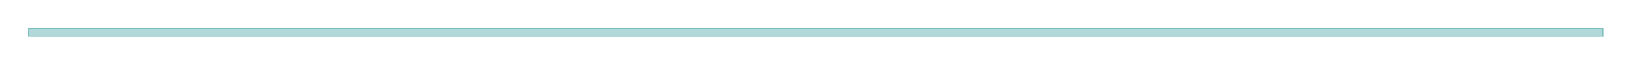
\begin{tikzpicture}[scale=1]
   \filldraw[teal, opacity=0.3](0,0)--(20,0)--(20,0.1)--(0,0.1)--cycle;
 \end{tikzpicture}

Row echelon form
\begin{expandable}
    A matrix is said to be in \dfn{row-echelon form} if:
\begin{enumerate}
\item All entries below each leading entry are 0.
\item Each leading entry is in a column to the right of the leading entries in the rows above it.
\item All rows of zeros, if there are any, are located below non-zero rows.
\end{enumerate}
\end{expandable}


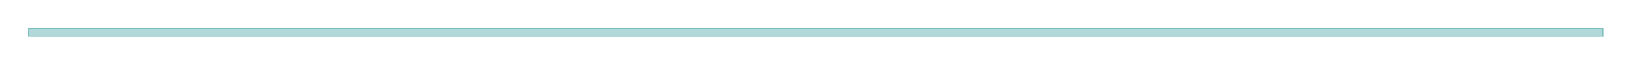
\begin{tikzpicture}[scale=1]
   \filldraw[teal, opacity=0.3](0,0)--(20,0)--(20,0.1)--(0,0.1)--cycle;
 \end{tikzpicture}

Row equivalent matrices
\begin{expandable}
    Two matrices $A$ and $B$ are said to be row equivalent if there is a sequence of elementary row operations that converts $A$ to $B$.
\end{expandable}


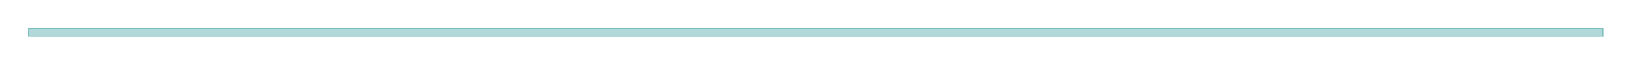
\begin{tikzpicture}[scale=1]
   \filldraw[teal, opacity=0.3](0,0)--(20,0)--(20,0.1)--(0,0.1)--cycle;
 \end{tikzpicture}


System of linear equations
Row equivalent matrices
\begin{expandable}
    A finite set of linear (degree 1) equations each with the same variables.
\end{expandable}


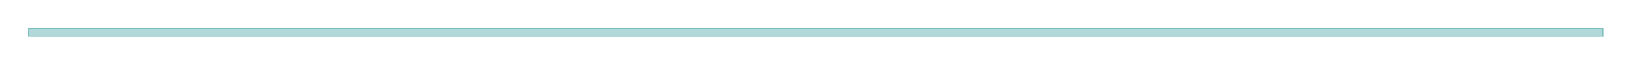
\begin{tikzpicture}[scale=1]
   \filldraw[teal, opacity=0.3](0,0)--(20,0)--(20,0.1)--(0,0.1)--cycle;
 \end{tikzpicture}

\end{document}
